\documentclass{article}

\usepackage{hyperref}
\usepackage{amsmath}
\usepackage{graphicx}
\usepackage{subcaption}
\usepackage{epstopdf}

\usepackage{times}

% Page layout
\hoffset -0in
\voffset -1in
\oddsidemargin 0in
\textheight 9.3in
\textwidth 6.3in

\setlength{\parindent}{0pt}
%\setlength{\intextsep}{10pt}
%\pagestyle{empty}

\graphicspath{{figures/}}

\begin{document}
	\section*{COMPUTATIONAL METHODS IN MECHANICS: Task 3}
	Vesa-Ville Hurskainen, 7 Feb 2018\\
	\href{https://github.com/VesaVilleHurskainen/cmim2018}{GitHub repository}

	\section*{Introduction}
	This is a report of the third assignment of the course \textit{Computational Methods in Mechanics}. The assignment consists of four tasks, which are as follows:
	
	\begin{enumerate}
		\setlength\itemsep{0pt}
		\item To use GitHub.
		\item To use the Symbolic Math Toolbox to create a plot of the forced vibration response for an amplitude.
		\item To write a function to create publication-quality plots and use it.
		\item To embed the plot in the report as vector graphics, with fonts of similar size and type as in the text itself.
	\end{enumerate}

	\section*{Methods}
	An ordinary mass-spring-damper system with a harmonic force excitation was studied, the equation of motion for which is as follows:
	\begin{equation}
		m \ddot{x} + c \dot{x} + k x = F \sin(\omega t)
	\end{equation}
	where $m$ is mass, $c$ is damping ratio, $k$ is spring stiffness, $F$ is force amplitude and $\omega$ is force frequency. The system was symbolically solved using the script \texttt{task03.m} and the results were plotted into figures. After being created, the figures were formatted using the function \texttt{formatplot.m}.

	\section*{Results}
	After being symbolically solved, the response of the system was plotted by substituting numeric parameters. For example, by substituting a set of parameters ($k$ = 10 N/m, $\omega = 2$ rad/s, $F$ = 10, damping ratio $\zeta = 0.5$ and undamped natural frequency $\omega_n$ = 2 rad/s) and removing all transient terms, the following steady state response function was created:
	\begin{equation}
		x_s(t) = - \cos(2t)
	\end{equation}
	Figure~\ref*{fig:response} illustrates the difference between the system response and it steady state part in this example.
		
	\begin{figure}[htb]
		\centering
		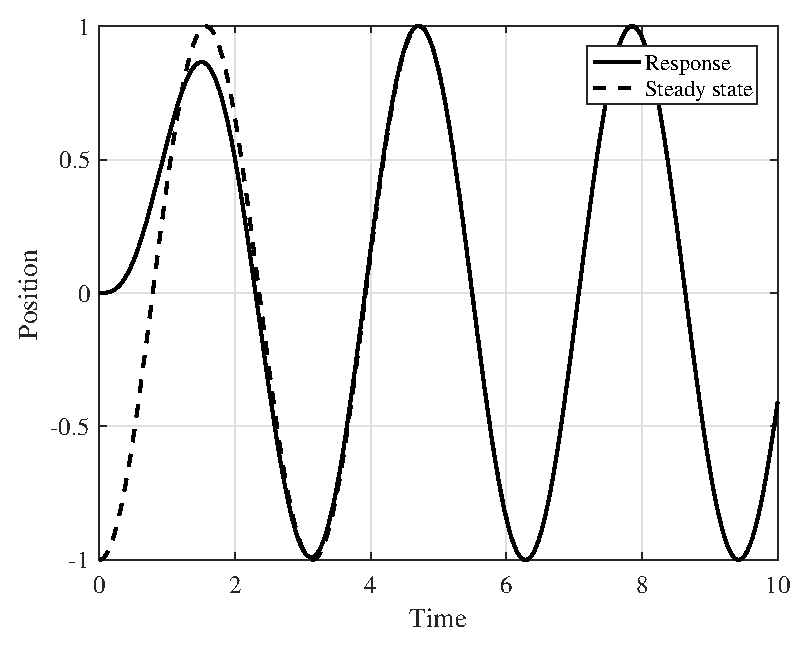
\includegraphics[width=0.5\textwidth]{response.eps}
		\caption{Comparison of total system response and its steady state part.}
		\label{fig:response}
	\end{figure}
	
	Figure~\ref{fig:steadystate} further illustrates the steady state response of the example system, by comparing the amplitude ratio and phase angle of the system to its frequency ratio, with different values for damping.
	
	\begin{figure}[htb]
		\centering
		\begin{subfigure}[t]{0.49\textwidth}
			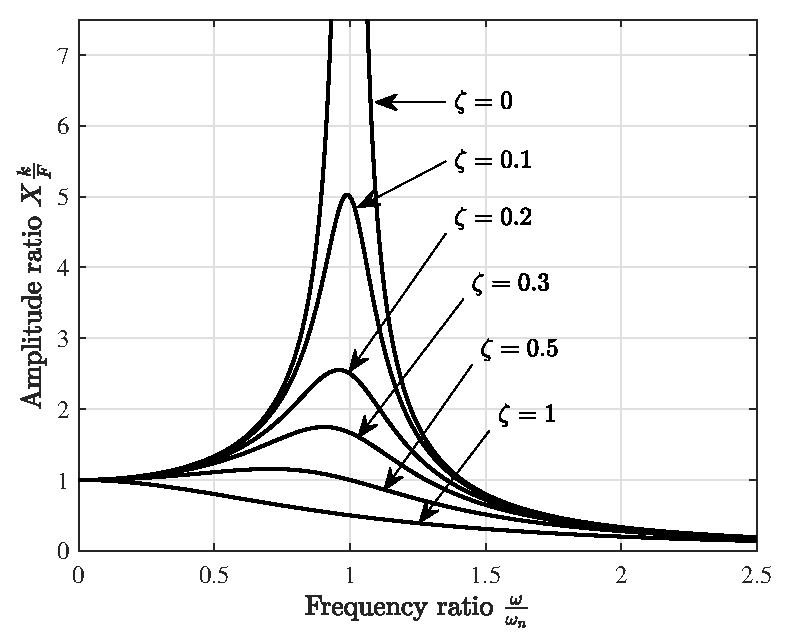
\includegraphics[width=\textwidth]{amplitude.eps}
			\caption{Amplitude ratio versus frequency ratio.}
		\end{subfigure}
		\begin{subfigure}[t]{0.49\textwidth}
			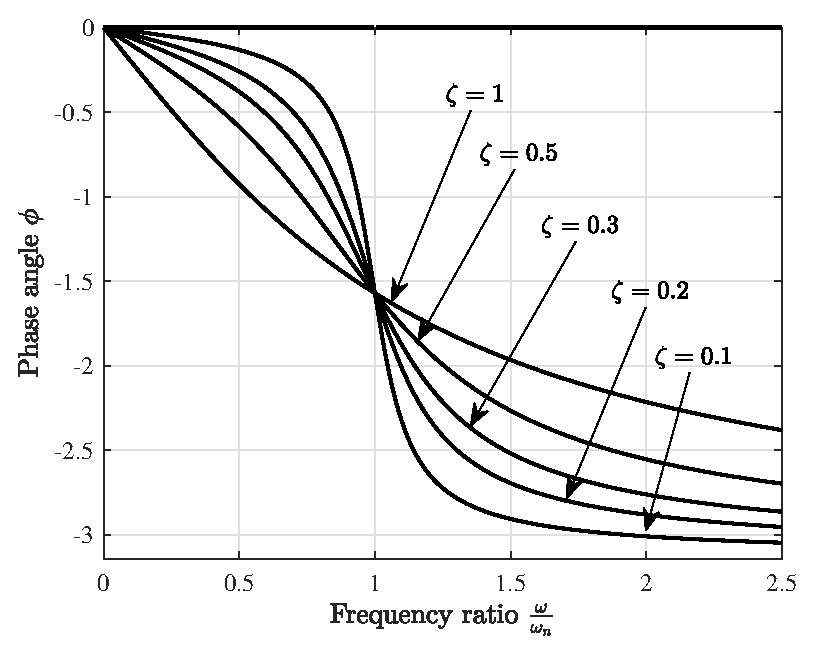
\includegraphics[width=\textwidth]{phaseangle.eps}
			\caption{Phase angle versus frequency ratio.}
		\end{subfigure}
		\caption{Comparison of system steady state responses.}
		\label{fig:steadystate}
	\end{figure}

	\section*{Analysis}
	Task one of the assignment was completed by managing the assignment files in the GitHub repository. Task two can be judged complete as well, since the script appears to function correctly and no problems were found in the results presented in Figure~\ref*{fig:steadystate}. The third task was completed by utilizing the function \texttt{formatplot.m} and the fourth and final task by importing the figures into this report in EPS format. Therefore, all tasks are complete.
	
\end{document}